\documentclass[a4paper, 12pt]{article}
\usepackage{custom}
\usepackage{pgfplots}
\pgfplotsset{compat=1.18} % Impostare la compatibilità con la versione installata


%--------------------VARIABILI--------------------
\def\lastversion{v0.3}
\def\title{Piano di qualifica}
\def\date{19 Febbraio 2025}
%------------------------------------------------

\begin{document}

\primapagina

\begin{registromodifiche}
       v0.3 & 19 Febbraio 2025 & Enrico Bianchi & Francesco Savio & Aggiornamento \hyperref[sec:cruscotti_qualità]{cruscotti di valutazione della qualità}\\
    \hline
       v0.2 & 7 gennaio 2025 & Enrico Bianchi & Marko Peric & aggiunte tabelle delle metriche nelle sezioni \hyperref[subsec:obiettivi_processo]{Qualità di processo}, \hyperref[subsec:obiettivi_prodotto]{Qualità di prodotto}, aggiunta sezione \hyperref[subsec:processi_metriche]{Metriche per processo} \\
    \hline
        v0.1 & 23 dicembre 2024  & Enrico Bianchi & Marko Peric & Sezioni \hyperref[sec:introduzione_pq]{Introduzione documento}, \hyperref[sec:obiettivi_qualità]{Introduzione obiettivi di qualità}\\
    \hline
\end{registromodifiche}

 \tableofcontents

\newpage



\subsection{Introduzione}
In questa sezione vengono elencati i requisiti software trovati dal gruppo per la realizzazione del progetto ArtificalQI.
I requisiti sono stati trovati tramite l'analisi degli use case individuati dal gruppo, dall'analisi del capitolato fornito dall'azienda e dalle riunioni esterne.
Ogni requisito software ha una nomenclatura composta come segue:
\begin{lstlisting}
    R[Tipologia]-[ID_RequisitoSoftware]
\end{lstlisting}
Dove:
\begin{enumerate}
    \item \lstinline|R| stà per requisito
    \item \lstinline|Tipologia| si divide in tre categorie
    \begin{enumerate}
        \item Funzionali (F): sono i requisiti software che soddisfano i comportamenti o le funzionalità del sistema.
        \item Qualitativi (Q): sono i requisiti software che servono per soddisfare gli standard qualitativi e di manutenibilità
        del prodotto software.
        \item Di Vincolo/Dominio (V): sono i requisiti che delineano le restrizione che gli Stakeholders o il capitolato impongono
         per la realizzazione del progetto software.
    \end{enumerate}
    \item \lstinline|ID_requisito| è un numero progressivo a partire da 0 che individua il requisito software.
\end{enumerate}  
Per ogni requisito software viene indicata una specifica che definisce i sotto requisiti di cui esso è composto.
L'identificazione dei sotto requisiti segue la nomeclatura:
\begin{lstlisting}
R[Tipologia]-[ID_RequisitoSoftware].[ID_SottoRequisito]
\end{lstlisting} 
Dove \lstinline|ID_SottoRequisito| è un numero progressivo a partire da 0 che identifica il sotto requisito.

\section{Obiettivi di qualità}
\label{sec:obiettivi_qualità}
Questa sezione ha lo scopo di indicare le metriche utilizzate per l'accertamento della qualità dei processi impiegati nella realizzazione
del progetto e dei prodotti realizzati.
Le metriche indicate si suddividono in:
\begin{itemize}
    \item metriche di processo
    \item metriche di prodotto
\end{itemize} 
Ogni metrica avrà indicato il codice identificativo associato, la soglia minima di accettazione e la soglia che ci si auspica di raggiungere 
per accertare la qualità massima raggiungibile dal processo o dal prodotto.
Ogni metrica indicata nelle tabelle realizzate è descritta con maggiore completezza all'interno del processo di Accertamento di Qualità nelle Norme di Progetto.

\subsection{Qualità di processo}
\label{subsec:obiettivi_processo}
La qualità di processo si riferisce all'efficacia con cui vengono implementati e gestiti i processi durante il ciclo di vita dello sviluppo software, 
con l'obiettivo di garantire che il prodotto finale soddisfi i requisiti prefissati. 
Per monitorare e migliorare i processi, vengono adottate metriche di processo, ovvero indicatori chiave che misurano l'efficienza, l'affidabilità 
e la conformità delle attività svolte. 
Questi parametri, selezionati dal team, consentono di identificare aree critiche, ottimizzare le procedure operative e migliorare la produttività complessiva. 
L'uso delle metriche di processo contribuisce al controllo della qualità e alla riduzione dei rischi associati a ritardi o difetti.


\begin{table}[H]
    \centering
    \begin{tabular}{| l | l | l | l |}
    \hline
    \textbf{Identificativo} & 
    \textbf{Nome} &
    \textbf{Valore ammissible} &
    \textbf{Valore ottimo}\\
    \hline
        M.PC.PV & Planned Value & $\geq 0$ & $\leq BAC$ \\
    \hline
        M.PC.EV & Earned Value & $\geq 0$ & $\leq EAC$ \\
    \hline
        M.PC.AC & Actual Cost & $\geq 0$ & $\leq EAC$ \\
    \hline
        M.PC.SV & Schedule Variance & $\geq -15\%$ & $0\%$ \\
    \hline
        M.PC.CV & Cost Variance & $\geq -15\%$ & $0\%$ \\
    \hline  
        M.PC.VP & \makecell{Variazione del Piano \\ tra costo effettivo \\ e costo preventivato} & $\leq 20\%$ & $\leq 5\%$ \\
    \hline
        M.PC.EAC & Estimated at Completion & $\leq BAC+5\% BAC$ & $\leq BAC$ \\
    \hline
        M.PC.RI & Rischi inattesi & $\leq 3$ & $0$ \\
    \hline
        M.PC.RMR & Risk Mitigation Rate & $\geq 75\%$ & $100\%$ \\
    \hline
        M.PC.MS & Metriche Soddisfatte & $\geq 75\%$ & $100\%$ \\
    \hline
    \end{tabular}
    \caption{Metriche di processo}
    \label{tab:metriche_processo} 
\end{table}

\subsection{Qualità di prodotto}
\label{subsec:obiettivi_prodotto}
La qualità di prodotto si riferisce al grado in cui un software soddisfa i requisiti specificati e le aspettative degli utenti.
Per valutarla vengono utilizzate metriche di prodotto, che rappresentano indicatori chiave per valutare le caratteristiche principali del software, che sono:
funzionalità, affidabilità, efficienza, usabilità, manutenibilità e portabilità.
Questi indicatori permettono di identificare lacune all'interno del codice permettendo un monitoraggio e un miglioramento continuo del prodotto
e assicurando che rispetti i requisiti funzionali e non funzionali prefissati.
L'adozione di metriche di prodotto permette quindi di assicurare la qualità del prodotto software realizzato e di ottimizzare l'esperienza 
dell'utente finale.

\begin{table}[H]
    \centering
    \resizebox{\textwidth}{!}{
    \begin{tabular}{| l | l | l | l |}
    \hline
        \textbf{Identificativo} & 
        \textbf{Nome} &
        \textbf{Valore ammissibile} &
        \textbf{Valore ottimo}\\
    \hline
        M.PR.PRM & Percentuale requisiti obbligatori soddisfatti & $100\%$ & $100\%$ \\
    \hline    
        M.PR.PRO & Percentuale requisiti opzionali soddisfatti & $\geq 0\%$ & $100\%$ \\
    \hline
        M.PR.CO & Correttezza Ortografica & $0$ & $0$ \\
    \hline
    \end{tabular}}
    \caption{Metriche di prodotto}
    \label{tab:metriche_prodotto} 
\end{table}

\subsubsection{Caratteristiche di prodotto}
Di seguito vengono elencate le metriche di prodotto associate a ciascuna delle caratteristiche generali descritte dallo standard ISO/IEC 9126, 
come indicato nel processo di Accertamento della Qualità nelle Norme di Progetto.
\begin{table}[H]
    \centering
    \begin{tabularx}{\textwidth}{| X | X | X |}
    \hline
        \textbf{Caratteristica} & 
        \textbf{Descrizione} &
        \textbf{Metriche associate}\\
    \hline
        Funzionalità & Capacità del software di fornire funzioni adatte a rispettare i requisiti sviluppati nel documento Analisi dei Requisiti & M.PR.PRM, M.PR.PRO \\
    \hline
        Affidabilità & Capacità del software di mantenere uno specificato livello di prestazioni in presenza di errori o malfunzionamenti & \\
    \hline
        Efficienza & Capacità del software di fornire appropriate prestazioni in relazione alle risorse usate & \\
    \hline
        Usabilità & Capacità del software di facilitare il reperimento delle informazioni dall'utente in modo che siano propriamente comprese & M.PR.CO, M.PR.IG \\
    \hline
        Manutenibilità & Facilità nella modifica del software per l'aggiunta di nuove funzionalità & \\
    \hline
        Portabilità & Capacità del software di essere adattato a differenti ambienti operativi & \\
    \hline
    \end{tabularx}
    \caption{Caratteristiche di prodotto}
    \label{tab:caratteristiche_prodotto} 
\end{table}







\subsection{Metriche per processo}
\label{subsec:processi_metriche}
Per ciascun processo delineato dallo standard ISO/IEC 12207 e descritto nel documento delle Norme di Progetto, 
vengono indicate le metriche di riferimento, se disponibili.

\subsubsection{Processi primari}
\paragraph{Fornitura}
\begin{table}[H]
    \centering
    \begin{tabular}{| l | l | l | l |}
    \hline
    \textbf{Identificativo} & 
    \textbf{Nome} &
    \textbf{Valore ammissibile} &
    \textbf{Valore ottimo}\\
    \hline
        M.PC.PV & Planned Value & $\geq 0$ & $\leq BAC$ \\
    \hline
        M.PC.EV & Earned Value & $\geq 0$ & $\leq EAC$ \\
    \hline
        M.PC.AC & Actual Cost & $\geq 0$ & $\leq EAC$ \\
    \hline
        M.PC.SV & Schedule Variance & $\geq -15\%$ & $0\%$ \\
    \hline
        M.PC.CV & Cost Variance & $\geq -15\%$ & $0\%$ \\
    \hline  
        M.PC.VP & Variazione del Piano & $\leq 20\%$ & $\leq 5\%$ \\
    \hline
        M.PC.EAC & Estimated at Completion & $\leq BAC+5\% BAC$ & $\leq BAC$ \\
    \hline
\end{tabular}
\caption{Metriche per processo di Fornitura}
\label{tab:metriche_fornitura} 
\end{table}

\paragraph{Sviluppo}
\begin{table}[H]
    \centering
    \begin{tabular}{| l | l | l | l |}
    \hline
    \textbf{Identificativo} & 
    \textbf{Nome} &
    \textbf{Valore ammissibile} &
    \textbf{Valore ottimo}\\
    \hline
        M.PR.PRM & \makecell{Percentuale requisiti \\ obbligatori soddisfatti} & $100\%$ & $100\%$ \\
    \hline
        M.PR.PRD & \makecell{Percentuale requisiti \\ desiderabili soddisfatti} & $\geq 25\%$ & $100\%$ \\
    \hline    
        M.PR.PRO & \makecell{Percentuale requisiti \\ opzionali soddisfatti} & $\geq 0\%$ & $100\%$ \\
    \hline
\end{tabular}
\caption{Metriche per processo di Sviluppo}
\label{tab:metriche_sviluppo} 
\end{table}

\subsubsection{Processi di supporto}
\paragraph{Documentazione}
\begin{table}[H]
    \centering
    \resizebox{\textwidth}{!}{
    \begin{tabular}{| l | l | l | l |}
    \hline
        \textbf{Identificativo} & 
        \textbf{Nome} &
        \textbf{Valore ammissibile} &
        \textbf{Valore ottimo}\\
    \hline
        M.PR.CO & Correttezza Ortografica & $0$ & $0$ \\
    \hline
\end{tabular}}
\caption{Metriche per processo di Documentazione}
\label{tab:metriche_documentazione} 
\end{table}

\paragraph{Accertamento della Qualità}
\begin{table}[H]
    \centering
    \resizebox{\textwidth}{!}{
    \begin{tabular}{| l | l | l | l |}
    \hline
        \textbf{Identificativo} & 
        \textbf{Nome} &
        \textbf{Valore ammissibile} &
        \textbf{Valore ottimo}\\
    \hline
        M.PC.MS & Metriche Soddisfatte & $\geq 75\%$ & $100\%$ \\
    \hline
\end{tabular}}
\caption{Metriche per processo di Accertamento della Qualità}
\label{tab:metriche_accertamento} 
\end{table}

\subsubsection{Processi Organizzativi}
\paragraph{Gestione dei Rischi}
\begin{table}[H]
    \centering
    \resizebox{\textwidth}{!}{
    \begin{tabular}{| l | l | l | l |}
    \hline
        \textbf{Identificativo} & 
        \textbf{Nome} &
        \textbf{Valore ammissibile} &
        \textbf{Valore ottimo}\\
    \hline
        M.PC.RMR & Risk Mitigation Rate & $\geq 75\%$ & $100\%$ \\
    \hline
\end{tabular}}
\caption{Metriche per processo di Gestione dei Rischi}
\label{tab:metriche_rischi} 
\end{table}



\section{Cruscotto di valutazione della qualità}
\subsection{M.PC.PV - Planned Value}

\begin{tikzpicture}
    \begin{axis}[
        width=12cm, height=8cm,
        ymin=0, ymax=11250,
        xtick={1, 2, 3},
        xticklabels={Sprint 1, Sprint 2, Sprint 3},
        xlabel={},
        ylabel={},
        grid=major,
        legend style={at={(0.5,1.05)}, anchor=south, legend columns=-1},
    ]
    \addplot coordinates {(1, 1125) (2, 3937.5), (3, 6187.5)};
    \addlegendentry{Valore misurato}
    \end{axis}
\end{tikzpicture}

\subsection*{RTB}

\subsection*{PB}
\subsection{M.PC.EV - Earned Value}

\begin{tikzpicture}
    \begin{axis}[
        width=12cm, height=8cm,
        ymin=0, ymax=11250,
        xtick={1, 2, 3},
        xticklabels={Sprint 1, Sprint 2, Sprint 3},
        xlabel={},
        ylabel={Costo (\euro)},
        grid=major,
        scaled ticks=false,
        legend style={at={(0.5,1.1)}, anchor=south, legend columns=-1},
    ]

    \pgfmathsetmacro{\EVA}{\BAC*\PercEA} 
    \pgfmathsetmacro{\EVB}{\BAC*\PercEB}
    \pgfmathsetmacro{\EVC}{\BAC*\PercEC} 

    \addplot coordinates {(1, \EVA) (2, \EVB) (3, \EVC)};
    \addlegendentry{Valore misurato}
    \addplot[red, thick] coordinates {(0, 0) (4, 0)};
    \addlegendentry{Valore ammissibile}
    \addplot[orange, thick] coordinates {(1, {\SpesaEA+(\BAC-\EVA)}) (2, {\SpesaEB+(\BAC-\EVB)}) (3, {\SpesaEC+(\BAC-\EVC)})};
    \addlegendentry{Valore ottimo}
    \end{axis}
\end{tikzpicture}

\subsection*{RTB}

\subsection*{PB}
\subsection{M.PC.AC - Actual Cost}

\begin{tikzpicture}
    \begin{axis}[
        width=12cm, height=8cm,
        ymin=0, ymax=12000,
        xtick={1, 2, 3},
        xticklabels={Sprint 1, Sprint 2, Sprint 3},
        xlabel={},
        ylabel={Costo (\euro)},
        grid=major,
        scaled ticks=false,
        legend style={at={(0.5,1.1)}, anchor=south, legend columns=-1},
    ]

    \pgfmathsetmacro{\EVA}{\BAC*\PercEA} 
    \pgfmathsetmacro{\EVB}{\BAC*\PercEB}
    \pgfmathsetmacro{\EVC}{\BAC*\PercEC} 

    \addplot coordinates {(1, \SpesaEA) (2, \SpesaEB) (3, \SpesaEC)};
    \addlegendentry{Valore misurato}
    \addplot[red, thick] coordinates {(0, 0) (4, 0)};
    \addlegendentry{Valore ammissibile}
    \addplot[orange, thick] coordinates {(1, {\SpesaEA+(\BAC-\EVA)}) (2, {\SpesaEB+(\BAC-\EVB)}) (3, {\SpesaEC+(\BAC-\EVC)})};
    \addlegendentry{Valore ottimo}
    \end{axis}
\end{tikzpicture}

\subsection*{RTB}

\subsection*{PB}
\subsection{M.PC.SV - Schedule Variance}

\begin{tikzpicture}
    \begin{axis}[
        width=12cm, height=8cm,
        ymin=-20, ymax=50,
        xtick={1, 2, 3},
        xticklabels={Sprint 1, Sprint 2, Sprint 3},
        xlabel={},
        ylabel={Percentuale (\%)},
        grid=major,
        scaled ticks=false,
        legend style={at={(0.5,1.1)}, anchor=south, legend columns=-1},
    ]
    \pgfmathsetmacro{\EVA}{\BAC*\PercEA} 
    \pgfmathsetmacro{\PVA}{\BAC*\PercTA}

    \pgfmathsetmacro{\EVB}{\BAC*\PercEB} 
    \pgfmathsetmacro{\PVB}{\BAC*\PercTB}

    \pgfmathsetmacro{\EVC}{\BAC*\PercEC} 
    \pgfmathsetmacro{\PVC}{\BAC*\PercTC}

    \addplot coordinates {(1, {((\EVA-\PVA)/\EVA)*100}) (2, {((\EVB-\PVB)/\EVB)*100}) (3, {((\EVC-\PVC)/\EVC)*100})};
    \addlegendentry{Valore misurato}
    \addplot[red, thick] coordinates {(0, -15) (4, -15)};
    \addlegendentry{Valore ammissibile}
    \addplot[orange, thick] coordinates {(0, 0) (4, 0)};
    \addlegendentry{Valore ottimo}
    \end{axis}
\end{tikzpicture}

\subsection*{RTB}

\subsection*{PB}
\subsection{M.PC.CV - Cost Variance}

\begin{tikzpicture}
    \begin{axis}[
        width=12cm, height=8cm,
        ymin=-50, ymax=100,
        xtick={1, 2},
        xticklabels={Sprint 1, Sprint 2},
        xlabel={},
        ylabel={},
        grid=major,
        legend style={at={(0.5,1.05)}, anchor=south, legend columns=-1},
    ]
    \addplot coordinates {(1, 10.3) (2, 58.8), (3, 67.6)};
    \addlegendentry{Valore misurato}
    \end{axis}
\end{tikzpicture}

\subsection*{RTB}

\subsection*{PB}
\subsection{M.PC.VP - Variazione del Piano}

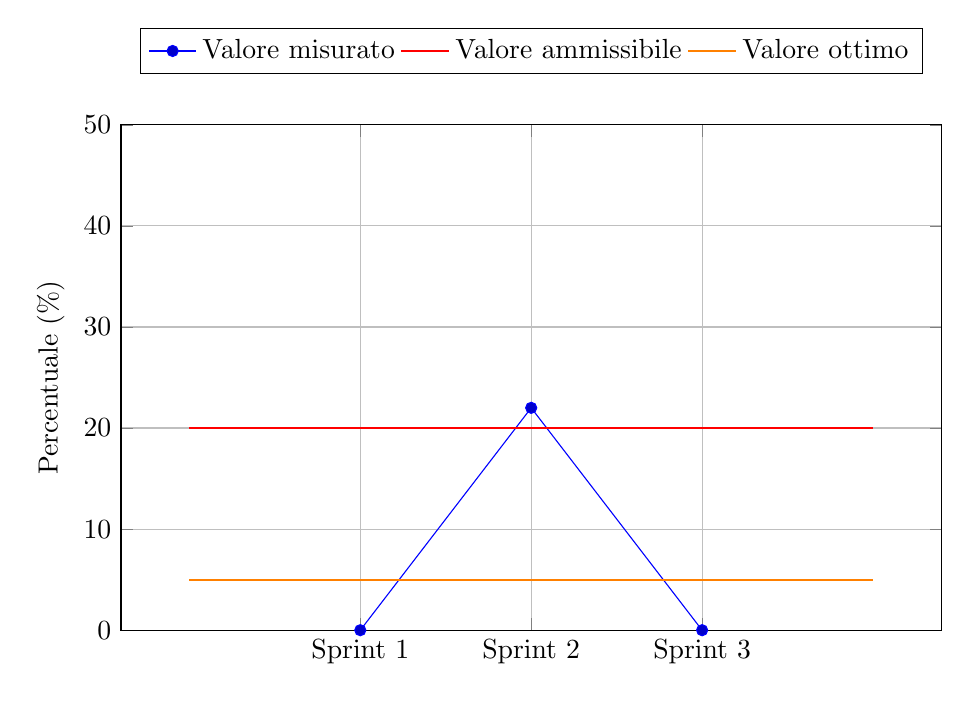
\begin{tikzpicture}
    \begin{axis}[
        width=12cm, height=8cm,
        ymin=0, ymax=50,
        xtick={1, 2, 3},
        xticklabels={Sprint 1, Sprint 2, Sprint 3},
        xlabel={},
        ylabel={Percentuale (\%)},
        grid=major,
        scaled ticks=false,
        legend style={at={(0.5,1.1)}, anchor=south, legend columns=-1},
    ]
    \addplot coordinates {(1, 0) (2, 22) (3, 0)};
    \addlegendentry{Valore misurato}
    \addplot[red, thick] coordinates {(0, 20) (4, 20)};
    \addlegendentry{Valore ammissibile}
    \addplot[orange, thick] coordinates {(0, 5) (4, 5)};
    \addlegendentry{Valore ottimo}
    \end{axis}
\end{tikzpicture}

\subsection*{RTB}

\subsection*{PB}
\subsection{M.PC.EAC - Estimated At Completition}

\begin{tikzpicture}
    \begin{axis}[
        width=12cm, height=8cm,
        ymin=0, ymax=14000,
        xtick={1, 2, 3},
        xticklabels={Sprint 1, Sprint 2, Sprint 3},
        xlabel={},
        ylabel={Costo (\euro)},
        grid=major,
        scaled ticks=false,
        legend style={at={(0.5,1.1)}, anchor=south, legend columns=-1},
    ]

    \pgfmathsetmacro{\EVA}{\BAC*\PercEA} 
    \pgfmathsetmacro{\EVB}{\BAC*\PercEB}
    \pgfmathsetmacro{\EVC}{\BAC*\PercEC} 

    \addplot coordinates {(1, {\SpesaEA+(\BAC-\EVA)}) (2, {\SpesaEB+(\BAC-\EVB)}) (3, {\SpesaEC+(\BAC-\EVC)})};
    \addlegendentry{Valore misurato}
    \addplot[red, thick] coordinates {(0, {\BAC + (\BAC*0.2)}) (4, {\BAC + (\BAC*0.2)})};
    \addlegendentry{Valore ammissibile}
    \addplot[orange, thick] coordinates {(0, \BAC) (4, \BAC)};
    \addlegendentry{Valore ottimo}
    \end{axis}
\end{tikzpicture}

\subsection*{RTB}

\subsection*{PB}
\subsection{M.PC.RI - Rischi Inattesi}

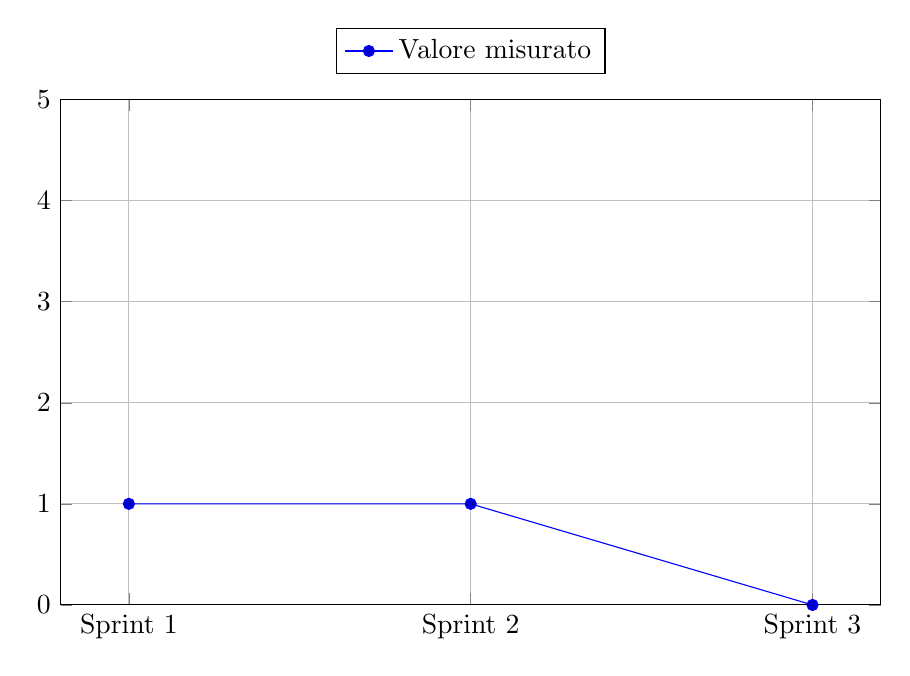
\begin{tikzpicture}
    \begin{axis}[
        width=12cm, height=8cm,
        ymin=0, ymax=5,
        xtick={1, 2, 3},
        xticklabels={Sprint 1, Sprint 2, Sprint 3},
        xlabel={},
        ylabel={},
        grid=major,
        legend style={at={(0.5,1.05)}, anchor=south, legend columns=-1},
    ]
    \addplot coordinates {(1, 1) (2, 1) (3, 0)};
    \addlegendentry{Valore misurato}
    \end{axis}
\end{tikzpicture}

\subsection*{RTB}

\subsection*{PB}
\subsection{M.PC.RMR - Risk Mitigation Rate}

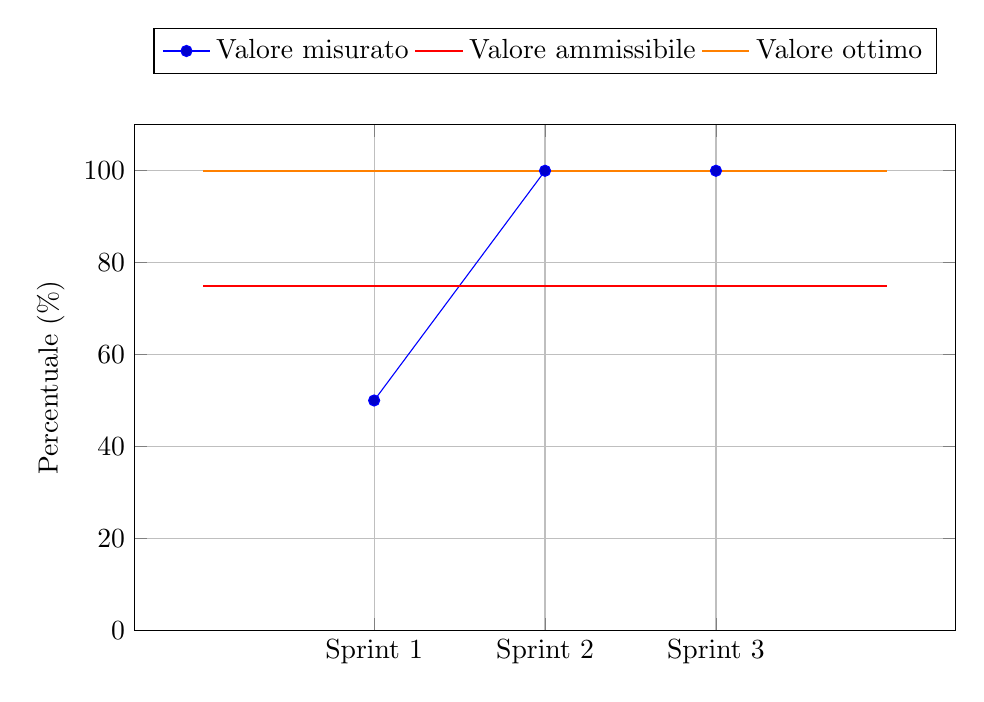
\begin{tikzpicture}
    \begin{axis}[
        width=12cm, height=8cm,
        ymin=0, ymax=110,
        xtick={1, 2, 3},
        xticklabels={Sprint 1, Sprint 2, Sprint 3},
        xlabel={},
        ylabel={Percentuale (\%)},
        grid=major,
        scaled ticks=false,
        legend style={at={(0.5,1.1)}, anchor=south, legend columns=-1},
    ]
    \addplot coordinates {(1, 50) (2, 100) (3, 100)};
    \addlegendentry{Valore misurato}
    \addplot[red, thick] coordinates {(0, 75) (4, 75)};
    \addlegendentry{Valore ammissibile}
    \addplot[orange, thick] coordinates {(0, 100) (4, 100)};
    \addlegendentry{Valore ottimo}
    \end{axis}
\end{tikzpicture}

\subsection*{RTB}

\subsection*{PB}
\subsection{M.PC.MS - Metriche Soddisfatte}

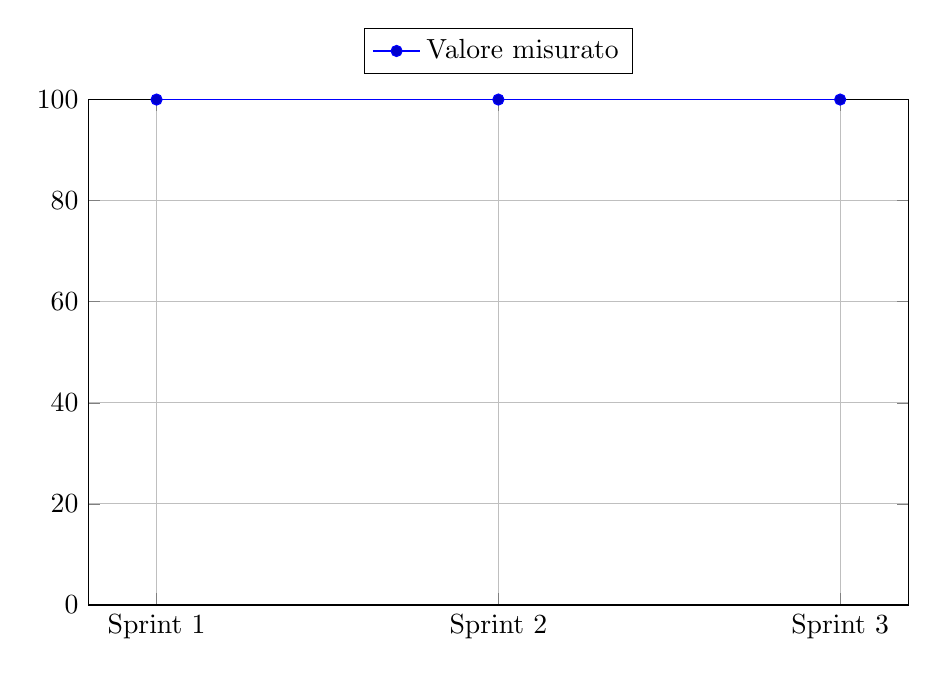
\begin{tikzpicture}
    \begin{axis}[
        width=12cm, height=8cm,
        ymin=0, ymax=100,
        xtick={1, 2, 3},
        xticklabels={Sprint 1, Sprint 2, Sprint 3},
        xlabel={},
        ylabel={},
        grid=major,
        legend style={at={(0.5,1.05)}, anchor=south, legend columns=-1},
    ]
    \addplot coordinates {(1, 100) (2, 100) (3, 100)};% ci vogliono prima i valori ammissibili e non, non sono sicuro della formula scritta su RTB/DocumentiInterni/NormeDiProgetto/Sezioni/ProcessiDiSupporto/Sottosezioni/AccertamentoQualità.tex riguardo le MetricheSoddisfatte
    \addlegendentry{Valore misurato}
    \end{axis}
\end{tikzpicture}

\subsection*{RTB}

\subsection*{PB}
\input{Sezioni/Cruscotto di valutazione della qualità/Sottosezioni/PercentualeRequisitiObbligatoriSoddisfatti.tex}
\subsection{M.PR.PRD - Percentuale Requisiti Desiderabili Soddisfatti}

\begin{tikzpicture}
    \begin{axis}[
        width=12cm, height=8cm,
        ymin=0, ymax=100,
        xtick={1, 2, 3},
        xticklabels={Sprint 1, Sprint 2, Sprint 3},
        xlabel={},
        ylabel={},
        grid=major,
        legend style={at={(0.5,1.05)}, anchor=south, legend columns=-1},
    ]
    \addplot coordinates {(1, 0) (2, 50), (3, 100)};
    \addlegendentry{Valore misurato}
    \end{axis}
\end{tikzpicture}

\subsection*{RTB}

\subsection*{PB}
\input{Sezioni/Cruscotto di valutazione della qualità/Sottosezioni/PercentualeRequisitiOpzionaliSoddisfatti.tex}
\subsection{M.PR.CO - Correttezza Ortografica}

\begin{tikzpicture}
    \begin{axis}[
        width=12cm, height=8cm,
        ymin=0, ymax=10,
        xtick={1, 2, 3},
        xticklabels={Sprint 1, Sprint 2, Sprint 3},
        xlabel={},
        ylabel={},
        grid=major,
        legend style={at={(0.5,1.05)}, anchor=south, legend columns=-1},
    ]
    \addplot coordinates {(1, 0) (2, 0), (3, 0)};
    \addlegendentry{Valore misurato}
    \end{axis}
\end{tikzpicture}

\subsection*{RTB}

\subsection*{PB}



\end{document}